\documentclass[]{article}
\usepackage{amsmath}
\usepackage{amssymb}
\usepackage{amsthm}
\usepackage{listings}
\usepackage{multirow}
\usepackage{tikz}
\usepackage{tikz-qtree}
\usepackage{tipa}
\usetikzlibrary{arrows,automata}
\begin{document}
\newcommand*{\xml}[1]{\texttt{<#1>}}
\theoremstyle{definition}
\newtheorem{thm}{Theorem}

\title{COMS W3261 \\ Computer Science Theory \\ Lecture 10\\ CNF, Pumping Lemma, 
CYK Algorithm}
\author{Alexander Roth}
\date{2014 -- 10 -- 06}
\maketitle

\section*{Outline}
  \begin{enumerate}
    \item Eliminating $\epsilon$-productions from a CFG
    \item Eliminating unit productions from a CFG
    \item Putting a CFG into Chomsky normal form
    \item Pumping lemma for CFL's
    \item Cocke-Younger-Kasami algorithm
  \end{enumerate}
    
\section{Eliminating $\epsilon$-productions from a CFG}
  \begin{itemize}
    \item If a language $L$ has a CFG, then $L - \{\epsilon\}$ has a CFG 
    without any $\epsilon$-productions.
    \item A nonterminal $A$ in a grammar is \emph{nullable} if $A \overset{*}
    {\Rightarrow} \epsilon$.
    \item The nullable nonterminals can be determined iteratively.
    \item We can eliminate all $\epsilon$-productions in a grammar as follows:
      \begin{itemize}
        \item Eliminate all productions with $\epsilon$ bodies.
        \item Suppose $A \rightarrow X_1X_2\ldots{}X_k$ is a production and $m$ 
        of the $kX_i$'s are nullable. Then add the $2^m$ versions of this 
        production where the nullable $X_i$'s are present or absent. (But if 
        all symbols are nullable, do not add an $\epsilon$-production.)
      \end{itemize}
    \item Let us eliminate the $\epsilon$-productions from the grammar $G$
      \begin{align*}
        S &\rightarrow AB \\
        A &\rightarrow aAA \, | \, \epsilon \\
        B &\rightarrow bBB \, | \, \epsilon \\
      \end{align*}
    $S$, $A$, and $B$ are nullable. \\
    For the production $S\rightarrow{AB}$ we add the productions $S
    \rightarrow{A} \, | \, B$ \\
    For the production $A\rightarrow{aAA}$ we add the productions $A
    \rightarrow{aA} \, | \, a$ \\
    For the production $B\rightarrow{bBB}$ we add the productions $B
    \rightarrow{bB} \, | \, b$ \\
    The resulting grammar $H$ with no $\epsilon$-production is
      \begin{align*}
        S &\rightarrow AB  \, | \,  A \, | \, B \\
        A &\rightarrow aAA \, | \, aA \, | \, a \\
        B &\rightarrow bBB \, | \, bB \, | \, b
      \end{align*}
    We can prove that $L(H) = L(G) - \{\epsilon\}$.
  \end{itemize}

\section{Eliminating Unit Productions from a CFG}
  \begin{itemize}
    \item A \emph{unit} production is one of the form $A \rightarrow B$ where 
    both $A$ and $B$ are nonterminals.
    \item Let us assume we are given a grammar $G$ with no 
    $\epsilon$-productions.
    \item From $G$ we can create an equivalent grammar $H$ with no unit 
    productions as follows.
      \begin{itemize}
        \item Define $(A, B)$ to be a unit pair if $A \overset{*}{\Rightarrow} 
        B$ in $G$.
        \item We can inductively construct all unit pairs for $G$.
        \item For each unit pair $(A,B)$ in $G$, we add to $H$ the productions 
        $A \rightarrow \alpha$ where $B \rightarrow \alpha$ is a nonunit 
        production of $G$.
      \end{itemize}
    \item Consider the standard grammar $G$ for arithmetic expressions:
      \begin{align*}
        E &\rightarrow E + T \, | \, T \\
        T &\rightarrow T * F \, | \, F \\
        F &\rightarrow ( E ) \, | \, a
      \end{align*}
    The unit pairs are $(E,E)$, $(E,T)$, $(E,F)$, $(T,T)$, $(T,F)$, $(F,F)$. \\
    The equivalent grammar $H$ with no unit productions is:
      \begin{align*}
        E &\rightarrow E + T \, | \, T * F \, | \, ( E ) \, | \, a \\
        T &\rightarrow T * F \, | \, ( E ) \, | \, a               \\
        F &\rightarrow ( E ) \, | \, a                             \\
      \end{align*}
  \end{itemize}
  
\section{Putting a CFG into Chomsky Normal Form}
  \begin{itemize}
    \item A grammar $G$ is in Chomsky Normal Form if each production in $G$ is 
    one of two forms:
      \begin{enumerate}
        \item $A \rightarrow BC$ where $A$, $B$, and $C$ are nonterminals, or
        \item $A \rightarrow a$ where $a$ is a terminal.
      \end{enumerate}
    \item We will further assume $G$ has no useless symbols.
    \item Every context-free language without $\epsilon$ can be generated by a 
    Chomsky Normal Form grammar.
    \item Let us assume we have a CFG $G$ with no useless symbols, $\epsilon$-
    productions, or unit productions. We can transform $G$ into an equivalent 
    Chomsky Normal Form grammar as follows:
      \begin{itemize}
        \item Arrange that all bodies of length two or more consist only of 
        nonterminals.
        \item Replace bodies of length three or more with a cascade of 
        productions, each with a body of two nonterminals.
      \end{itemize}
    \item Applying these two transformations to the grammar $H$ above, we get:
      \begin{align*}
        E &\rightarrow EA \, | \, TB \, | \, LC \, | a \\
        A &\rightarrow PT                              \\
        P &\rightarrow +                               \\
        B &\rightarrow MF                              \\
        M &\rightarrow *                               \\
        L &\rightarrow (                               \\
        C &\rightarrow ER                              \\
        R &\rightarrow )                               \\
        T &\rightarrow TB \, | \, LC \, | \, a         \\
        F &\rightarrow LC \, | \, a                    \\
      \end{align*}
  \end{itemize}
  \subsection*{Class Notes}
    Let $G$ be a CFG with no useless symbols, no $\epsilon$-productions, and no
    unit productions.
      \begin{align*}
        S &\rightarrow +SS \, | \, *SS \, | \, a \\
        S &\rightarrow PSS \, | \, TSS \, | \, a \\
        P &\rightarrow +                         \\
        T &\rightarrow *                         \\
        S &\rightarrow PA  \, | \, TA  \, | \, a \\
        A &\rightarrow SS                        \\
      \end{align*}
      \begin{thm}
        Let $G$ be a CFG in CNF. Suppose $w$ is in $L(G)$. If the length of a
        longest path in a parse tree for $w$ is of length $n$, then $|w|$ is 
        $2^{n-1}$ 
      \end{thm}
    If we break up the string $w$ into $xy$, then the length of $x$ and $y$
    subtrees is $|x| \leq 2^{n-2}$ and $|y| \leq 2^{n-2}$.
  
\section{Pumping Lemma for CFL's}
  \begin{itemize}
    \item For every nonfinite context-free language $L$, there exists a 
    constant $n$ that depends on $L$ such that for all $z$ in $L$ with $|z| 
    \geq n$, we can write $z$ as $uvwxy$ where
      \begin{enumerate}
        \item $vx \neq \epsilon$,
        \item $|vwx| \leq n$, and
        \item for all $i \geq 0$, the string $uv^iwx^iy$ is in $L$.
      \end{enumerate}
    \item Proof: See HMU, pp 281 -- 282.
    \item One important use of the pumping lemma is to prove certain languages 
    are not context free.
    \item Example: The language $L = \{a^nb^nc^n \, | \, n \geq 0 \}$ is not 
    context free.
      \begin{itemize}
        \item The proof will be by contradiction. Assume $L$ is context free. 
        Then by the pumping lemma there is a constant $n$ associated with $L$ 
        such that for all $z$ in $L$ with $|z| \geq n$, $z$ can be written as 
        $uvwxy$ such that
          \begin{enumerate}
            \item $vx \neq \epsilon$,
            \item $|vwx| \leq n$, and 
            \item for all $i \geq 0$, the string $uv^iwx^iy$ is in $L$.
          \end{enumerate}
        \item Consider the string $z = a^nb^nc^n$.
        \item From condition (2), $vwx$ cannot contain both $a$'s and $c$'s.
        \item Two cases arise:
          \begin{enumerate}
            \item $vwx$ has no $c$'s. But then $uwy$ cannot be in $L$ since at 
            least one of $v$ or $x$ is nonempty.
            \item $vwx$ has no $a$'s. Again, $uwy$ cannot be in $L$.
          \end{enumerate}
        In both cases we have a contradiction, so we must conclude $L$ cannot 
        be context free. The details of the proof can be found in HMU, p. 284.
      \end{itemize}
  \end{itemize}

\section{Cocke-Younger-Kasami Algorithm for Testing Membership in a CFL}
  \begin{itemize}
    \item Input: a Chomsky normal form CFG $G = (V,T,P,S)$ and a string $w = 
    a_1a_2\ldots{a_n}$ in $T^*$.
    \item Output: ``yes'' if $w$ is in $L(G)$, ``no'' otherwise.
    \item Method: The CYK algorithm is a dynamic programming algorithm that 
    fils in a triangular table $x_{ij}$ with nonterminals $A$ such that $A 
    \overset{*}{\Rightarrow} a_ia_i+j\ldots{a_j}$.
      \begin{figure}[p]
        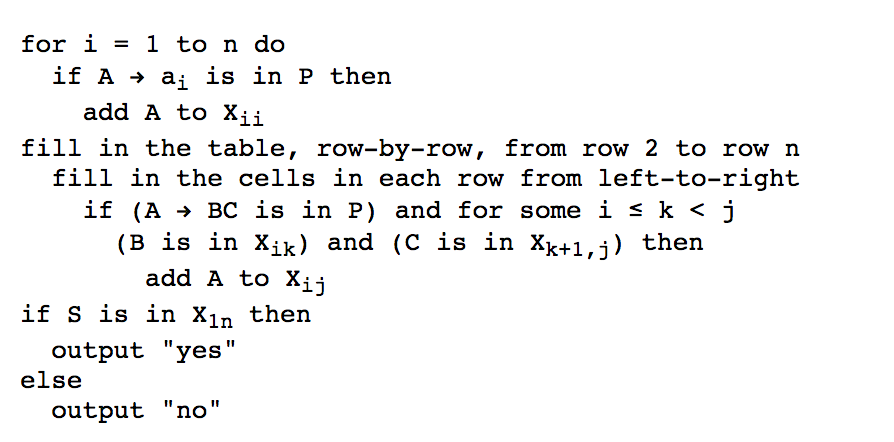
\includegraphics{./img/CYK_Algorithm.png}
        \caption{The CYK Algorithm in Pseudocode}
      \end{figure}
    \item The algorithm adds nonterminal $A$ to $x_{ij}$ iff there is a 
    production $A \rightarrow BC$ in $P$ where $B \overset{*}{\Rightarrow}
    a_ia_{i+1}\ldots{a_k}$ and $C \overset{*}{\Rightarrow}a_{k+1}a_{k
    +2}\ldots{a_j}$.
    \item To compute entry $x_{ij}$, we examine at most $n$ pairs of entries: 
    $(x_{ii},x_{i+1},_j)$,$(x_i,_{i+1},x_{i+2},_j)$, and so on until $
    (x_i,_{j-1},x_{j},_j)$.
    \item The running time of the CYK algorithm is $O(n^3)$.
  \end{itemize}
\end{document}